\chapter{作物模式}
%\addcontentsline{toc}{chapter}{作物模式}

%\begin{作物模式}
GPAM1可以模拟作物生长发育的关键过程及其对天气/气候、近地面大气CO2和O3浓度和氮沉降、
农田管理的响应和生物、化学、物理反馈(图\ref{fig:作物模式GPAM1框图})。
图\ref{fig:作物模式GPAM1框图}中蓝色高亮部分为作物区别与自然植被、需要特殊处理的过程。
{
\begin{figure}[]
\centering
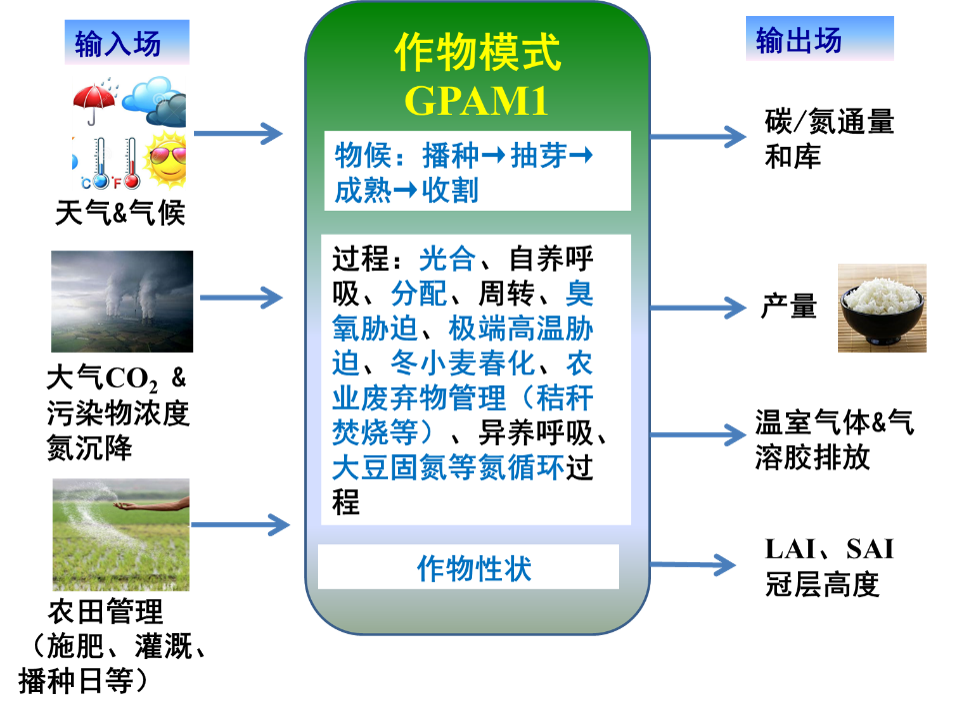
\includegraphics{Figures/作物模式/作物模式GPAM1框图.png}
\caption{作物模式GPAM1框图。  }
\label{fig:作物模式GPAM1框图}
\end{figure}
}
\section{作物功能类型(CFT)}
GPAM1包含10个作物功能类型(Crop Functional Type, CFT),模拟4种作物类型: 小麦、水稻、玉米、大豆(图\ref{fig:作物功能类型覆盖率的空间分布})。
每种作物类型各分雨养(rainfed)和灌溉(irrigated) CFT,小麦又分冬小麦和春小麦。每个CFT占用一个水热独立的陆表单元(patch)。
{
\begin{figure}[]
\centering
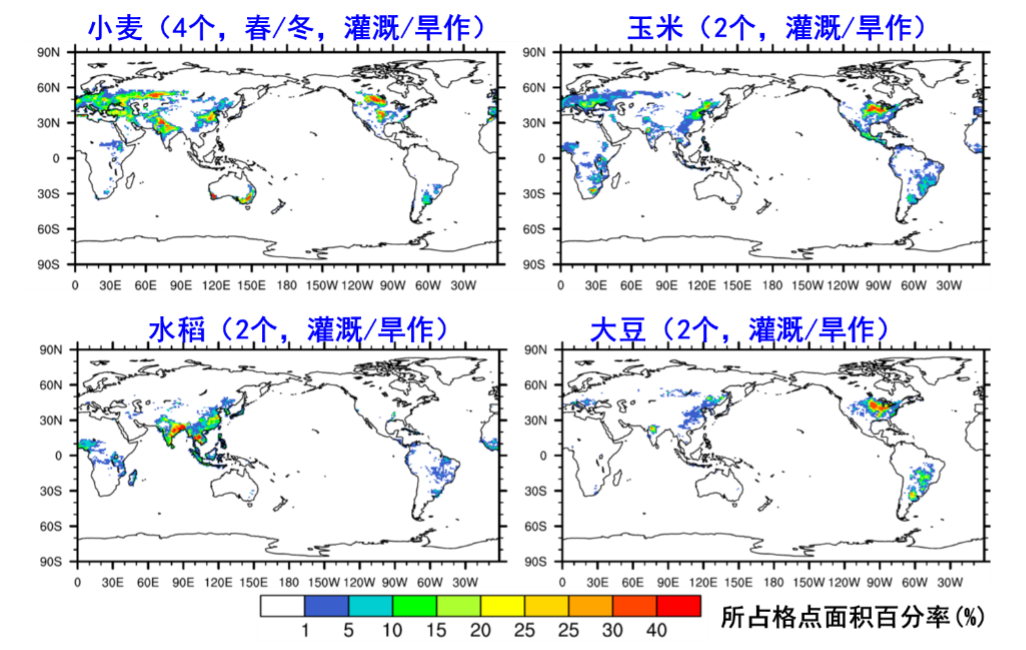
\includegraphics{Figures/作物模式/作物功能类型覆盖率的空间分布.png}
\caption{GPAM1模式模拟的10个作物功能类型(CFT)覆盖率的空间分布。}
\label{fig:作物功能类型覆盖率的空间分布}
\end{figure}
}
\section{物候}
GPAM1的物候包括三个阶段: (1)播种->抽芽; (2)抽芽到开始灌浆(grain fill); (3)灌浆到成熟/收割。所涉及的参数取值见表 \ref{tab:作物物候方案相关参数}。\\
\begin{enumerate}
  \item 播种\\
  播种日期是给定的,采用全球播种日再分析数据(Jägermeyr et al., in prep.),并结合陆表数据中的作物分布制作而成,为GPAM1的输入场。
  \item 抽芽\\
  当热单元指数(Heat Unit Index, $HUI$):
  \begin{equation}\label{HUI}
  HUI=\frac{GDD_{base}}{GDD_{mat}}
  \end{equation}
  达到$f_{LE}$时,开始抽芽。$GDD_{base}$是基于陆表气温的积温($^{\circ}$C days):
  \begin{equation}
  GDD_{ {base }}=\sum_{planting}^{currentday} \min \left(0, T_{sa}-T_{base}\right)
  \end{equation}
  公式中(\ref{HUI}),$T_sa$是日地表气温,$T_{base}$是底温(作物在该温度下停止生长)。\\
  \item 灌浆\\
  当$HUI$达到$f_{GF}$时,开始灌浆。
  \item 成熟\\
  当$HUI$达到1时或生长季达到最长生长季长度$GSL_{max}$时,作物成熟。其中,$GDD_{mat}$是$GDD_{base}$ 
  10年滑动平均的一元线性方程(表\ref{tab:作物物候方案相关参数})。
  \begin{equation}
    GDD_{mat}=a GDD_{10yr}+b
  \end{equation}
  \item 收割\\
  假设达到成熟的时步收割。
\end{enumerate}
% Please add the following required packages to your document preamble:
% \usepackage{booktabs}
\begin{table}[]
  \centering
  \caption{作物物候方案相关参数}
  \label{tab:作物物候方案相关参数}
\begin{tabular}{@{}cccccc@{}}
\toprule
    & $T_{base}$ & $f_{LE}$  & $f_{GF}$  & $GDD_{mat}$          & $GSL_{max}$ \\ \midrule
春小麦 & 0     & 0.07 & 0.60 & 0.2$GDD_{10yr}$+1458 & 150    \\
冬小麦 & 0     & 0.03 & 0.67 & 0.38$GDD_{10yr}$+526 & 270    \\
水稻1 & 10    & 0.12 & 0.68 & 0.30$GDD_{10yr}$+695 & 150    \\
水稻2 & 10    & 0.35 & 0.75 & 0.27$GDD_{10yr}$+575 & 150    \\
玉米  & 8     & 0.11 & 0.64 & 0.26$GDD_{10yr}$r+907 & 150    \\
大豆  & 10    & 0.15 & 0.69 & 0.26$GDD_{10yr}$+802 & 150    \\ \bottomrule
\end{tabular}
\end{table}

\section{分配}
分配系数随物候阶段变化而变化。从出叶开始,按下列分配系数公式分配到叶库Cleaf,茎库Cleaf,根库Croot,粒库Cgrain。
不同物候期分配系数见表\ref{tab:作物分配方案相关参数}。

(1)	物候期2 \\
\begin{equation}
\left\{\begin{array}{c}
  a_{grain}=0 \\ 
  a_{root}=a_{root_i}-\left(a_{root_i}-a_{root_f}\right) HUI \\
  a_{leaf}=\left(1-a_{root}\right) a_{leaf_i} \frac{{e}^{-{b}}-{e}^{-b \frac{H U I}{f_{GF}}}}{{e}^{-{b}}-1}   \\
  a_{stem}=1-a_{ {grain }}-a_{ {root }}-a_{ {leaf }}\end{array}\right.
\end{equation}
其中,下标$i$和$f$表示该分配系数的初值和终值,$b=0.1$。

(2)	物候期3 \\
\begin{equation}
  \left\{\begin{array}{c}
    a_{leaf}=0.0 \\ 
    a_{root}=a_{root_i}-\left(a_{root_i}-a_{root_f}\right) \min(1, HUI) \\
    a_{stem}=\max \left[a_{stem_f}, a_{stem} \max \left(0, \frac{1-HUI}{1-f_{GF}}\right)^{d_{sem}}\right. \\
    a_{grain}=1-a_{root}-a_{leaf}-a_{stem}\end{array}\right.
\end{equation}
% Please add the following required packages to your document preamble:
% \usepackage{booktabs}
\begin{table}[]
  \centering
  \caption{作物分配方案相关参数}
  \label{tab:作物分配方案相关参数}
\begin{tabular}{@{}lcccc@{}}
  \toprule
参数       & 小麦   & 水稻   & 玉米   & 大豆   \\ \midrule
$\alpha_{leaf_i}$ & 0.9  & 0.75 & 0.8  & 0.85 \\
$\alpha_{root_i}$ & 0.1  & 0.1  & 0.4  & 0.2  \\
$\alpha_{root_f}$ & 0    & 0    & 0.05 & 0.2  \\
$\alpha_{stem_f}$ & 0.05 & 0.05 & 0.0  & 0.3  \\
$d_stem$    & 1    & 1    & 2    & 5   \\\bottomrule
\end{tabular}
\end{table}
\section{收割和农业残留物处理}
收割时粒库$C_{grain}$进入种子库$C_{seed}$和食品库$C_{food}$
\begin{equation}
{C}_{ {seed }}=\min \left({C}_{ {grain }}, 3\right)
\end{equation}
\begin{equation}
{C}_{ {food }}={C}_{ {grain }}-{C}_{ {seed }}
\end{equation}
其中,种子库$C_{seed}$在下一个生长季出叶期的第一时步转移到叶库$C_{leaf}$。叶和茎的碳库进入地上凋落物库。根的碳库进入地下凋落物库。


\section{氮循环}
作物的氮循环和自然植被类似,但碳氮比(CN)不同,且要考虑大豆生物固氮的特殊性和施肥。

(1) 碳氮比(CN)\\
表\ref{tab:作物碳氮比}中,碳氮比$CN_{leaf}$,$ CN_{stem}$, $CN_{root}$用于灌浆前,其余碳氮比用于灌浆开始后。\\
% Please add the following required packages to your document preamble:
% \usepackage{booktabs}
\begin{table}[]
  \centering
  \caption{作物碳氮比}
  \label{tab:作物碳氮比}
\begin{tabular}{@{}lcccc@{}}
\toprule
参数         & 小麦  & 水稻  & 玉米  & 大豆  \\ \midrule
$CN_{leaf}$     & 20  & 20  & 25  & 20  \\
$CN_{stem}$     & 50  & 50  & 50  & 50  \\
$CN_{root}$     & 42  & 42  & 42  & 42  \\
$CN_{leaf_f}$  & 65  & 65  & 65  & 65  \\
$CN_{stem_f}$  & 100 & 100 & 120 & 130 \\
$CN_{root_f}$  & 40  & 40  & 0   & 0   \\
$CN_{grain_f}$ & 50  & 50  & 50  & 50  \\ \bottomrule
\end{tabular}
\end{table}

(2) 大豆共生固氮 (SNF)\\
考虑大豆根瘤中的根瘤菌与大豆共生固氮,大豆共生固氮能力设为自然植物的4倍,假设其余作物类型无生物共生固氮能力。生物共生固定的氮直接被植物吸收。\\

(3) 施肥\\
氮肥考虑了工业氮肥和粪肥。工业氮肥是输入场。粪肥设为2 g $\rm N/m^2/yr$。
施肥时直接将氮肥输入土壤$NH_4^{+}$库,从出叶开始,以匀速的方式施肥20天。


\section{光合作用和气孔导度}
大豆、小麦、水稻采用C3植物光合方案;玉米采用C4植物光合方案。
在基于Medlyn方案计算气孔导度时,玉米的参数取值$g_1=1.8$,低于自然植被,其余作物的参数取值$g_1=5.8$,高于自然植被。该参数越大,气孔导度越高。


\section{臭氧污染胁迫}
考虑臭氧对光合速率和气孔导度的影响因子 $F_{O3_A}$ 以及$F_{O3_{gs}}$:
\begin{equation}
F_{O3_{A}}=-0.058 \log _{10}\left(POD_{0.5}\right)+0.883
\end{equation}
\begin{equation}
F_{O3_{gs}}=-0.109 \tanh \left(POD_{0.5}\right)+0.951
\end{equation}
其中,$POD_{0.5}$ (Phytotoxic ozone does above a threshold of 0.5 $nmol m^{-2} s^{-1}$,  单位:mmol $\rm m^{-2}$)是植物吸收的$O_3$通量累积量:
\begin{equation}
POD_{0.5}=\sum_{t}\left(\left[{O}_{3}\right] \times g_{s} \times D-0.5\right)
\end{equation}
在公式(15.10)中,$\left[{O}_{3}\right]$为陆面大气的臭氧浓度,$g_{s}$为叶气孔导度,
$D=0.663$为臭氧和水蒸气的扩散比,$t$是作物暴露在臭氧污染的时间,从抽芽开始。
上面计算的$F_{{O3}_A}$ 以及$F_{O3_{gs}}$分别作用在Farquhar-Collatz方案计算的光合速率以及Medlyn或Ball-Berry方案计算出的气孔导度。


\section{冬小麦春化现象}
春化响应$V$(0$\sim$1)采用\citet{streck2003incorporating}方案:
\begin{equation}
V=\frac{D_{v}{ }^{5}}{22.5^{5}+D_{v}^{5}}
\end{equation}
其中,$D_v$是物候阶段2累积的日春化率:
\begin{equation}\label{D_v_a}
D_{v}=\sum R_{v}
\end{equation}
在公式(\ref{D_v_a})中,$R_{v}$是日地表温度的函数:
\begin{equation}
R_{v}=\left\{\begin{array}{c}\frac{\left[2\left(T-T_{\min }\right)^{a}\left(T_{{opt}}-T_{\min }\right)^{a}-\left(T-T_{\min }\right)^{2 a}\right]}{\left(T_{{opt}}-T_{\min }\right)^{2 a}} \ \ \ \ \ \ \ \ \    T_{\min } \leq T \leq T_{\max }\\
 0   \ \ \  \ \ \ \ \ \ \ \ \ \    \ \ \ \ \   \ \ \ \ \ \ \ \ \ \ \ \ \ \ \  \ \ \ \ \    T<T_{\min } \quad  { or } \quad T>T_{\max }
\end{array}\right.
\end{equation}
其中,$T_{min}$= –1.3 \textcelsius, $T_{opt}$= 4.9 \textcelsius, $T_{max}$= 15.7 \textcelsius。$ R_v$ 的取值从 0 (当$ T\leq Tmin$ or $ \geq  Tmax$) 到 1 ( 当$T=T_{opt}$)。
\begin{equation}
a=\frac{\ln 2}{\ln \left[\left(T_{\max }-T_{\min }\right) /\left(T_{o p t}-T_{\min }\right)\right]}
\end{equation}
春化响应用于调整$GDD_{base}$和粒分配系数
\begin{equation}
G D D_{b a s e}=G D D_{b a s e,  { unadjusted }} \times V
\end{equation}
\begin{equation}
a_{ {grain }}=a_{ {grain,unadjusted }} \times V_{f}
\end{equation}


\section{热胁迫}
作物对热胁迫的敏感期大约是在开花前后及灌浆期,在GPAM1里设为$HUI $满足$0.5 \leq HUI \leq 0.8$的时段。在每个发生热胁迫的时步,采用场数损失率$l$:
\begin{equation}
l=\left\{\begin{array}{cc}1-\left(\frac{4.3}{10.4}\right)^{\frac{\Delta t}{3600^{*} 21}}, & T>T_{c} \\ 0, & T \leq T_{c}\end{array}\right.
\end{equation}
其中,$\Delta t$ 是时步长,$T$是该时步的温度;$T_c$是临界温度:$T_c$=34 \textcelsius (水稻,玉米,冬小麦),31 \textcelsius (春小麦),37 \textcelsius (大豆)。
每个时步考虑了热胁迫后的叶$C_{leaf}$库为:
\begin{equation}
C_{leaf}=C_{leaf,  {unadjusted}} \times l
\end{equation}


\section{秸秆焚烧及排放}
年燃烧面积百分率BAF来自GFED4s农田燃烧面积百分率观测数据,为输入场。火发生是根据GFED4s的3小时数据找到的燃烧顶峰时步中心点,为输入场。

在得到燃烧面积后,火灾引起的碳排放$CE$(g C $\rm m^{-2} s^{-1}$) 为:
\begin{equation}
CE=BAF \times C_{ab,litter} \times CC
\end{equation}
$C_{ab,litter}$是地上凋落物碳库, $CC=0.8$是燃烧完全因子。

此后,我们估算火灾引起的33种痕量气体和气溶胶排放。火灾引起的第$i$类痕量气体和气溶胶排放量$E_i$ ($\rm g species m^{-2} s^{-1}$):
\begin{equation}
E_{i}=EF_{i} \times CE /[{C}]
\end{equation}
$EF_i$(g species (kg dry matter (DM))$^{-1}$)是排放因子,见表\ref{tab:秸秆焚烧排放因子取值}。$[C]=0.5×10^3$ $\rm g C (kg DM)^{-1}$是单位转换因子。


% Please add the following required packages to your document preamble:
% \usepackage{booktabs}
\begin{table}[]
  \centering
  \caption{秸秆焚烧排放因子取值(g species $(kg DM)^{-1}$)}
  \label{tab:秸秆焚烧排放因子取值}
  \begin{tabular}{@{}lccc@{}}
  \toprule
  \multicolumn{1}{c}{种类} & 排放因子 & 种类                     & 排放因子 \\ \midrule
  CO2                    & 1421 & C2H4   (ethylene)      & 1.14 \\
  CO                     & 78   & C3H6   (propylene)     & 0.48 \\
  CH4                    & 5.9  & C5H8   (isoprene)      & 0.18 \\
  NMHC                   & 5.8  & C10H16   (terpenes)    & 0.03 \\
  H2                     & 2.65 & C7H8   (toluene)       & 0.18 \\
  NOx                    & 2.67 & C6H6   (benzene)       & 0.31 \\
  N2O                    & 0.09 & C8H10   (xylene)       & 0.09 \\
  PM2.5                  & 8.5  & CH2O   (formaldehyde)  & 1.80 \\
  TPM                    & 11.3 & C2H4O   (acetaldehyde) & 1.82 \\
  TPC                    & 5.5  & C3H6O   (acetone)      & 0.61 \\
  OC                     & 5.0  & C3H6O2(hydroxyacetone) & 1.74 \\
  BC                     & 0.43 & C6H5OH   (Phenol)      & 0.50 \\
  SO2                    & 0.81 & NH3 (ammonia)          & 1.04 \\
  C2H6   (ethane)        & 0.76 & HCN (hydrogen cyanide) & 0.43 \\
  CH3OH   (methanol)     & 2.63 & MEK/2-butanone         & 0.60 \\
  C3H8   (propane)       & 0.20 & CH3CN   (acetonitrile) & 0.25 \\
  C2H2   (acetylene)     & 0.32 &                        &      \\ \bottomrule
  \end{tabular}
  \end{table}


\section{灌溉}
灌溉水直接进入到达地表的水,不经过截流。灌溉包括两个方案:
\begin{enumerate}
  \item 灌溉量和灌溉时间为输入场;
  \item CLM5灌溉模型。
\end{enumerate}
\section{结构形态}
出叶后到收割前,叶面积为:
\begin{equation}
LAI=C_{leaf} \times SLA
\end{equation}
SLA为比叶面积 ($\rm m^2 leaf g^{-1} C$)(表\ref{tab:结构形态参数})。

茎叶面积为:
\begin{equation}
SAI=\left\{\begin{array}{lcc}0.1 LAI, & \text { for } & \text { maize } \\
   0.2 LAI, & \text { for } & \text {others}\end{array}\right.
\end{equation}

冠层顶高度$z_{top}$(米)和冠层底高度$z_{bot}$(米)为:
\begin{equation}
z_{top}=\max \left[0.05, z_{\max} \min \left(\frac{GDD_{base}}{f_{GE} G D D_{mat}}, 1.0\right)\right]
\end{equation}
\begin{equation}
z_{b o t}=0.02
\end{equation}

% Please add the following required packages to your document preamble:
% \usepackage{booktabs}
\begin{table}[]
  \centering
  \caption{结构形态参数}
  \label{tab:结构形态参数}
  \begin{tabular}{@{}ccccc@{}}
  \toprule
  参数   & 小麦   & 水稻    & 玉米   & 大豆    \\ \midrule
  $SLA$  & 0.05 & 0.035 & 0.05 & 0.035 \\
  $zmax$ & 1    & 1.5   & 3    & 1     \\ \bottomrule
  \end{tabular}
\end{table}
